\documentclass[twoside]{book}

% Packages required by doxygen
\usepackage{fixltx2e}
\usepackage{calc}
\usepackage{doxygen}
\usepackage[export]{adjustbox} % also loads graphicx
\usepackage{graphicx}
\usepackage[utf8]{inputenc}
\usepackage{makeidx}
\usepackage{multicol}
\usepackage{multirow}
\PassOptionsToPackage{warn}{textcomp}
\usepackage{textcomp}
\usepackage[nointegrals]{wasysym}
\usepackage[table]{xcolor}

% Font selection
\usepackage[T1]{fontenc}
\usepackage[scaled=.90]{helvet}
\usepackage{courier}
\usepackage{amssymb}
\usepackage{sectsty}
\renewcommand{\familydefault}{\sfdefault}
\allsectionsfont{%
  \fontseries{bc}\selectfont%
  \color{darkgray}%
}
\renewcommand{\DoxyLabelFont}{%
  \fontseries{bc}\selectfont%
  \color{darkgray}%
}
\newcommand{\+}{\discretionary{\mbox{\scriptsize$\hookleftarrow$}}{}{}}

% Page & text layout
\usepackage{geometry}
\geometry{%
  a4paper,%
  top=2.5cm,%
  bottom=2.5cm,%
  left=2.5cm,%
  right=2.5cm%
}
\tolerance=750
\hfuzz=15pt
\hbadness=750
\setlength{\emergencystretch}{15pt}
\setlength{\parindent}{0cm}
\setlength{\parskip}{3ex plus 2ex minus 2ex}
\makeatletter
\renewcommand{\paragraph}{%
  \@startsection{paragraph}{4}{0ex}{-1.0ex}{1.0ex}{%
    \normalfont\normalsize\bfseries\SS@parafont%
  }%
}
\renewcommand{\subparagraph}{%
  \@startsection{subparagraph}{5}{0ex}{-1.0ex}{1.0ex}{%
    \normalfont\normalsize\bfseries\SS@subparafont%
  }%
}
\makeatother

% Headers & footers
\usepackage{fancyhdr}
\pagestyle{fancyplain}
\fancyhead[LE]{\fancyplain{}{\bfseries\thepage}}
\fancyhead[CE]{\fancyplain{}{}}
\fancyhead[RE]{\fancyplain{}{\bfseries\leftmark}}
\fancyhead[LO]{\fancyplain{}{\bfseries\rightmark}}
\fancyhead[CO]{\fancyplain{}{}}
\fancyhead[RO]{\fancyplain{}{\bfseries\thepage}}
\fancyfoot[LE]{\fancyplain{}{}}
\fancyfoot[CE]{\fancyplain{}{}}
\fancyfoot[RE]{\fancyplain{}{\bfseries\scriptsize Generated by Doxygen }}
\fancyfoot[LO]{\fancyplain{}{\bfseries\scriptsize Generated by Doxygen }}
\fancyfoot[CO]{\fancyplain{}{}}
\fancyfoot[RO]{\fancyplain{}{}}
\renewcommand{\footrulewidth}{0.4pt}
\renewcommand{\chaptermark}[1]{%
  \markboth{#1}{}%
}
\renewcommand{\sectionmark}[1]{%
  \markright{\thesection\ #1}%
}

% Indices & bibliography
\usepackage{natbib}
\usepackage[titles]{tocloft}
\setcounter{tocdepth}{3}
\setcounter{secnumdepth}{5}
\makeindex

% Custom commands
\newcommand{\clearemptydoublepage}{%
  \newpage{\pagestyle{empty}\cleardoublepage}%
}

\usepackage{caption}
\captionsetup{labelsep=space,justification=centering,font={bf},singlelinecheck=off,skip=4pt,position=top}

%===== C O N T E N T S =====

\begin{document}

% Titlepage & ToC
\pagenumbering{alph}
\begin{titlepage}
\vspace*{7cm}
\begin{center}%
{\Large S.\+L.\+K (Simple . Ludic . Kernel) \\[1ex]\large 1.\+0 }\\
\vspace*{1cm}
{\large Generated by Doxygen 1.8.13}\\
\end{center}
\end{titlepage}
\clearemptydoublepage
\pagenumbering{roman}
\tableofcontents
\clearemptydoublepage
\pagenumbering{arabic}

%--- Begin generated contents ---
\chapter{File Index}
\section{File List}
Here is a list of all documented files with brief descriptions\+:\begin{DoxyCompactList}
\item\contentsline{section}{/home/raz0ntex/\+Desktop/slk/src/\textbf{ kernel.\+c} \\*Kernel\textquotesingle{}s main file }{\pageref{kernel_8c}}{}
\item\contentsline{section}{/home/raz0ntex/\+Desktop/slk/src/libk/includes/\textbf{ stdint.\+h} \\*Kernel\textquotesingle{}s basic types }{\pageref{stdint_8h}}{}
\end{DoxyCompactList}

\chapter{File Documentation}
\section{/home/raz0ntex/\+Desktop/slk/src/kernel.c File Reference}
\label{kernel_8c}\index{/home/raz0ntex/\+Desktop/slk/src/kernel.\+c@{/home/raz0ntex/\+Desktop/slk/src/kernel.\+c}}


Kernel\textquotesingle{}s main file.  


{\ttfamily \#include \char`\"{}libk/includes/stdint.\+h\char`\"{}}\newline
Include dependency graph for kernel.\+c\+:
\nopagebreak
\begin{figure}[H]
\begin{center}
\leavevmode
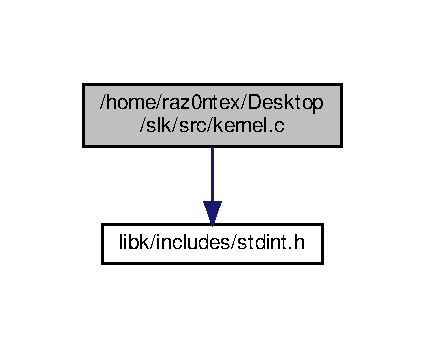
\includegraphics[width=204pt]{kernel_8c__incl}
\end{center}
\end{figure}
\subsection*{Enumerations}
\begin{DoxyCompactItemize}
\item 
enum \textbf{ vga\+\_\+color} \{ \newline
{\bfseries V\+G\+A\+\_\+\+C\+O\+L\+O\+R\+\_\+\+B\+L\+A\+CK} = 0, 
{\bfseries V\+G\+A\+\_\+\+C\+O\+L\+O\+R\+\_\+\+B\+L\+UE} = 1, 
{\bfseries V\+G\+A\+\_\+\+C\+O\+L\+O\+R\+\_\+\+G\+R\+E\+EN} = 2, 
{\bfseries V\+G\+A\+\_\+\+C\+O\+L\+O\+R\+\_\+\+C\+Y\+AN} = 3, 
\newline
{\bfseries V\+G\+A\+\_\+\+C\+O\+L\+O\+R\+\_\+\+R\+ED} = 4, 
{\bfseries V\+G\+A\+\_\+\+C\+O\+L\+O\+R\+\_\+\+M\+A\+G\+E\+N\+TA} = 5, 
{\bfseries V\+G\+A\+\_\+\+C\+O\+L\+O\+R\+\_\+\+B\+R\+O\+WN} = 6, 
{\bfseries V\+G\+A\+\_\+\+C\+O\+L\+O\+R\+\_\+\+L\+I\+G\+H\+T\+\_\+\+G\+R\+EY} = 7, 
\newline
{\bfseries V\+G\+A\+\_\+\+C\+O\+L\+O\+R\+\_\+\+D\+A\+R\+K\+\_\+\+G\+R\+EY} = 8, 
{\bfseries V\+G\+A\+\_\+\+C\+O\+L\+O\+R\+\_\+\+L\+I\+G\+H\+T\+\_\+\+B\+L\+UE} = 9, 
{\bfseries V\+G\+A\+\_\+\+C\+O\+L\+O\+R\+\_\+\+L\+I\+G\+H\+T\+\_\+\+G\+R\+E\+EN} = 10, 
{\bfseries V\+G\+A\+\_\+\+C\+O\+L\+O\+R\+\_\+\+L\+I\+G\+H\+T\+\_\+\+C\+Y\+AN} = 11, 
\newline
{\bfseries V\+G\+A\+\_\+\+C\+O\+L\+O\+R\+\_\+\+L\+I\+G\+H\+T\+\_\+\+R\+ED} = 12, 
{\bfseries V\+G\+A\+\_\+\+C\+O\+L\+O\+R\+\_\+\+L\+I\+G\+H\+T\+\_\+\+M\+A\+G\+E\+N\+TA} = 13, 
{\bfseries V\+G\+A\+\_\+\+C\+O\+L\+O\+R\+\_\+\+L\+I\+G\+H\+T\+\_\+\+B\+R\+O\+WN} = 14, 
{\bfseries V\+G\+A\+\_\+\+C\+O\+L\+O\+R\+\_\+\+W\+H\+I\+TE} = 15
 \}\begin{DoxyCompactList}\small\item\em Define hardware text mode for console. \end{DoxyCompactList}
\end{DoxyCompactItemize}
\subsection*{Functions}
\begin{DoxyCompactItemize}
\item 
\mbox{\label{kernel_8c_ab8ff83f1c6edb3ab0e2119686167dcef}} 
\textbf{ uint16\+\_\+t} \textbf{ strlen} (const char $\ast$str)
\begin{DoxyCompactList}\small\item\em Give the length of str. \end{DoxyCompactList}\item 
void \textbf{ terminal\+\_\+initialize} (void)
\begin{DoxyCompactList}\small\item\em Initialize terminal. \end{DoxyCompactList}\item 
void \textbf{ terminal\+\_\+setcolor} (\textbf{ uint8\+\_\+t} color)
\begin{DoxyCompactList}\small\item\em Set the terminal color. \end{DoxyCompactList}\item 
void \textbf{ terminal\+\_\+putentryat} (char c, \textbf{ uint8\+\_\+t} color, \textbf{ uint16\+\_\+t} x, \textbf{ uint16\+\_\+t} y)
\begin{DoxyCompactList}\small\item\em Write char at an entry of V\+GA buffer. \end{DoxyCompactList}\item 
void \textbf{ terminal\+\_\+putchar} (char c)
\begin{DoxyCompactList}\small\item\em Write a char without specifying its dimension and color. \end{DoxyCompactList}\item 
void \textbf{ terminal\+\_\+write} (const char $\ast$data, \textbf{ uint16\+\_\+t} size)
\begin{DoxyCompactList}\small\item\em Write a string. \end{DoxyCompactList}\item 
\mbox{\label{kernel_8c_a09ed5506d8ae907e2c8e0c96f6d1a928}} 
void \textbf{ terminal\+\_\+writestring} (const char $\ast$data)
\begin{DoxyCompactList}\small\item\em Write a string. \end{DoxyCompactList}\item 
\mbox{\label{kernel_8c_a6b8fb674fb359f6ae53dc9c4fb7fc6be}} 
void {\bfseries kernel\+\_\+main} (void)
\end{DoxyCompactItemize}
\subsection*{Variables}
\begin{DoxyCompactItemize}
\item 
\mbox{\label{kernel_8c_a8bb65c78998dc43716e51c11a38e23d6}} 
\textbf{ uint8\+\_\+t} {\bfseries terminal\+\_\+row}
\item 
\mbox{\label{kernel_8c_adfadf4bb39940ae59774731f41520ff8}} 
\textbf{ uint8\+\_\+t} {\bfseries terminal\+\_\+column}
\item 
\mbox{\label{kernel_8c_a0165452ad102b2a781847d6616407976}} 
\textbf{ uint8\+\_\+t} {\bfseries terminal\+\_\+color}
\item 
\mbox{\label{kernel_8c_a47e72657e89c79ddc7393b941112a28e}} 
\textbf{ uint16\+\_\+t} $\ast$ {\bfseries terminal\+\_\+buffer}
\end{DoxyCompactItemize}


\subsection{Detailed Description}
Kernel\textquotesingle{}s main file. 

\begin{DoxyAuthor}{Author}
wil.\+tor
\end{DoxyAuthor}
 \begin{DoxyDate}{Date}
31/10/2018
\end{DoxyDate}
\begin{DoxyVersion}{Version}
1.\+0
\end{DoxyVersion}
Write in V\+GA\textquotesingle{}s buffer. 

\subsection{Enumeration Type Documentation}
\mbox{\label{kernel_8c_abaae057bae62d0c3e11501e3199cb60e}} 
\index{kernel.\+c@{kernel.\+c}!vga\+\_\+color@{vga\+\_\+color}}
\index{vga\+\_\+color@{vga\+\_\+color}!kernel.\+c@{kernel.\+c}}
\subsubsection{vga\+\_\+color}
{\footnotesize\ttfamily enum \textbf{ vga\+\_\+color}}



Define hardware text mode for console. 

Define programmable 16 color palette of V\+GA text mode. 

\subsection{Function Documentation}
\mbox{\label{kernel_8c_ac4802010a838e2e4909fe47fc7edbe3e}} 
\index{kernel.\+c@{kernel.\+c}!terminal\+\_\+initialize@{terminal\+\_\+initialize}}
\index{terminal\+\_\+initialize@{terminal\+\_\+initialize}!kernel.\+c@{kernel.\+c}}
\subsubsection{terminal\+\_\+initialize()}
{\footnotesize\ttfamily void terminal\+\_\+initialize (\begin{DoxyParamCaption}\item[{void}]{ }\end{DoxyParamCaption})}



Initialize terminal. 

Initialize the properties of termine by accessing the vga buffer at the 0x\+B8000 address with a size for 80x25 characters. \mbox{\label{kernel_8c_a0e77ef8710654966af44f69becffcd80}} 
\index{kernel.\+c@{kernel.\+c}!terminal\+\_\+putchar@{terminal\+\_\+putchar}}
\index{terminal\+\_\+putchar@{terminal\+\_\+putchar}!kernel.\+c@{kernel.\+c}}
\subsubsection{terminal\+\_\+putchar()}
{\footnotesize\ttfamily void terminal\+\_\+putchar (\begin{DoxyParamCaption}\item[{char}]{c }\end{DoxyParamCaption})}



Write a char without specifying its dimension and color. 


\begin{DoxyParams}{Parameters}
{\em c} & The char to write in V\+GA buffer. \\
\hline
\end{DoxyParams}
\mbox{\label{kernel_8c_a6df85b4463bee56146ea4e16c13d6708}} 
\index{kernel.\+c@{kernel.\+c}!terminal\+\_\+putentryat@{terminal\+\_\+putentryat}}
\index{terminal\+\_\+putentryat@{terminal\+\_\+putentryat}!kernel.\+c@{kernel.\+c}}
\subsubsection{terminal\+\_\+putentryat()}
{\footnotesize\ttfamily void terminal\+\_\+putentryat (\begin{DoxyParamCaption}\item[{char}]{c,  }\item[{\textbf{ uint8\+\_\+t}}]{color,  }\item[{\textbf{ uint16\+\_\+t}}]{x,  }\item[{\textbf{ uint16\+\_\+t}}]{y }\end{DoxyParamCaption})}



Write char at an entry of V\+GA buffer. 

Write char by specifying its dimensions and its color.


\begin{DoxyParams}{Parameters}
{\em c} & The char to push.\\
\hline
{\em color} & The color to set at char c.\\
\hline
{\em x} & The width of char c.\\
\hline
{\em y} & The height of char c. \\
\hline
\end{DoxyParams}
\mbox{\label{kernel_8c_a1d0c38c1fb48053bea2c7f60cbd3ccb9}} 
\index{kernel.\+c@{kernel.\+c}!terminal\+\_\+setcolor@{terminal\+\_\+setcolor}}
\index{terminal\+\_\+setcolor@{terminal\+\_\+setcolor}!kernel.\+c@{kernel.\+c}}
\subsubsection{terminal\+\_\+setcolor()}
{\footnotesize\ttfamily void terminal\+\_\+setcolor (\begin{DoxyParamCaption}\item[{\textbf{ uint8\+\_\+t}}]{color }\end{DoxyParamCaption})}



Set the terminal color. 

  
\begin{DoxyParams}{Parameters}
{\em color} & The color to set at terminal. \\
\hline
\end{DoxyParams}
\mbox{\label{kernel_8c_a6844c7f6acece37baec90ab8da52d0c4}} 
\index{kernel.\+c@{kernel.\+c}!terminal\+\_\+write@{terminal\+\_\+write}}
\index{terminal\+\_\+write@{terminal\+\_\+write}!kernel.\+c@{kernel.\+c}}
\subsubsection{terminal\+\_\+write()}
{\footnotesize\ttfamily void terminal\+\_\+write (\begin{DoxyParamCaption}\item[{const char $\ast$}]{data,  }\item[{\textbf{ uint16\+\_\+t}}]{size }\end{DoxyParamCaption})}



Write a string. 

Write the first \textquotesingle{}size\textquotesingle{} bytes of the strings \textquotesingle{}data\textquotesingle{}.


\begin{DoxyParams}{Parameters}
{\em data} & The string to write.\\
\hline
{\em size} & The number of bytes of \textquotesingle{}data\textquotesingle{} string to be written. \\
\hline
\end{DoxyParams}

\section{/home/raz0ntex/\+Desktop/slk/src/libk/includes/stdint.h File Reference}
\label{stdint_8h}\index{/home/raz0ntex/\+Desktop/slk/src/libk/includes/stdint.\+h@{/home/raz0ntex/\+Desktop/slk/src/libk/includes/stdint.\+h}}


Kernel\textquotesingle{}s basic types.  


This graph shows which files directly or indirectly include this file\+:
\nopagebreak
\begin{figure}[H]
\begin{center}
\leavevmode
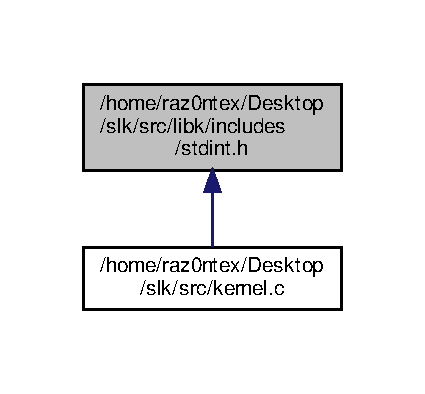
\includegraphics[width=204pt]{stdint_8h__dep__incl}
\end{center}
\end{figure}
\subsection*{Macros}
\begin{DoxyCompactItemize}
\item 
\mbox{\label{stdint_8h_aadcf2a81af243df333b31efa6461ab8e}} 
\#define \textbf{ I\+N\+T8\+\_\+\+M\+IN}~(-\/128)
\begin{DoxyCompactList}\small\item\em Define mininmum value for int8\+\_\+t type. \end{DoxyCompactList}\item 
\mbox{\label{stdint_8h_ad4e9955955b27624963643eac448118a}} 
\#define \textbf{ I\+N\+T16\+\_\+\+M\+IN}~(-\/32768)
\begin{DoxyCompactList}\small\item\em Define mininmum value for int16\+\_\+t type. \end{DoxyCompactList}\item 
\mbox{\label{stdint_8h_a688eb21a22db27c2b2bd5836943cdcbe}} 
\#define \textbf{ I\+N\+T32\+\_\+\+M\+IN}~(-\/2147483648)
\begin{DoxyCompactList}\small\item\em Define minimum value for int32\+\_\+t type. \end{DoxyCompactList}\item 
\mbox{\label{stdint_8h_aaf7f29f45f1a513b4748a4e5014ddf6a}} 
\#define \textbf{ I\+N\+T8\+\_\+\+M\+AX}~127
\begin{DoxyCompactList}\small\item\em Define maximum value for int8\+\_\+t type. \end{DoxyCompactList}\item 
\mbox{\label{stdint_8h_ac58f2c111cc9989c86db2a7dc4fd84ca}} 
\#define \textbf{ I\+N\+T16\+\_\+\+M\+AX}~32767
\begin{DoxyCompactList}\small\item\em Define maximum value for int16\+\_\+t type. \end{DoxyCompactList}\item 
\mbox{\label{stdint_8h_a181807730d4a375f848ba139813ce04f}} 
\#define \textbf{ I\+N\+T32\+\_\+\+M\+AX}~2147483647
\begin{DoxyCompactList}\small\item\em Define maximum value for int32\+\_\+t type. \end{DoxyCompactList}\item 
\mbox{\label{stdint_8h_aeb4e270a084ee26fe73e799861bd0252}} 
\#define \textbf{ U\+I\+N\+T8\+\_\+\+M\+AX}~255
\begin{DoxyCompactList}\small\item\em Define maximum value for uint8\+\_\+t type. \end{DoxyCompactList}\item 
\mbox{\label{stdint_8h_a3ea490c9b3617d4479bd80ef93cd5602}} 
\#define \textbf{ U\+I\+N\+T16\+\_\+\+M\+AX}~65535
\begin{DoxyCompactList}\small\item\em Define maximum value for int16\+\_\+t type. \end{DoxyCompactList}\item 
\mbox{\label{stdint_8h_ab5eb23180f7cc12b7d6c04a8ec067fdd}} 
\#define \textbf{ U\+I\+N\+T32\+\_\+\+M\+AX}~4294967295
\begin{DoxyCompactList}\small\item\em Define maximul value for int32\+\_\+t type. \end{DoxyCompactList}\end{DoxyCompactItemize}
\subsection*{Typedefs}
\begin{DoxyCompactItemize}
\item 
\mbox{\label{stdint_8h_aef44329758059c91c76d334e8fc09700}} 
typedef signed char \textbf{ int8\+\_\+t}
\begin{DoxyCompactList}\small\item\em Define int8\+\_\+t type as an exact 8-\/bit value. \end{DoxyCompactList}\item 
\mbox{\label{stdint_8h_aba7bc1797add20fe3efdf37ced1182c5}} 
typedef unsigned char \textbf{ uint8\+\_\+t}
\begin{DoxyCompactList}\small\item\em Define uint8\+\_\+t type as an exact 8-\/bit value. \end{DoxyCompactList}\item 
\mbox{\label{stdint_8h_a269259c924dce846340ddbb810db2e3c}} 
typedef signed short \textbf{ int16\+\_\+t}
\begin{DoxyCompactList}\small\item\em Define int16\+\_\+t type as an exact 16-\/bit value. \end{DoxyCompactList}\item 
\mbox{\label{stdint_8h_a273cf69d639a59973b6019625df33e30}} 
typedef unsigned short \textbf{ uint16\+\_\+t}
\begin{DoxyCompactList}\small\item\em Define uint16\+\_\+t type as an exact 16-\/bit value. \end{DoxyCompactList}\item 
\mbox{\label{stdint_8h_ab1967d8591af1a4e48c37fd2b0f184d0}} 
typedef signed int \textbf{ int32\+\_\+t}
\begin{DoxyCompactList}\small\item\em Define int32\+\_\+t type as an exact 32-\/bit value. \end{DoxyCompactList}\item 
\mbox{\label{stdint_8h_a435d1572bf3f880d55459d9805097f62}} 
typedef unsigned int \textbf{ uint32\+\_\+t}
\begin{DoxyCompactList}\small\item\em Define uint32\+\_\+t type as an exact 32-\/bit value. \end{DoxyCompactList}\end{DoxyCompactItemize}


\subsection{Detailed Description}
Kernel\textquotesingle{}s basic types. 

\begin{DoxyAuthor}{Author}
wil.\+tor
\end{DoxyAuthor}
 \begin{DoxyDate}{Date}
29/10/2018
\end{DoxyDate}
\begin{DoxyVersion}{Version}
1.\+0
\end{DoxyVersion}
Define basics int types. 
%--- End generated contents ---

% Index
\backmatter
\newpage
\phantomsection
\clearemptydoublepage
\addcontentsline{toc}{chapter}{Index}
\printindex

\end{document}
